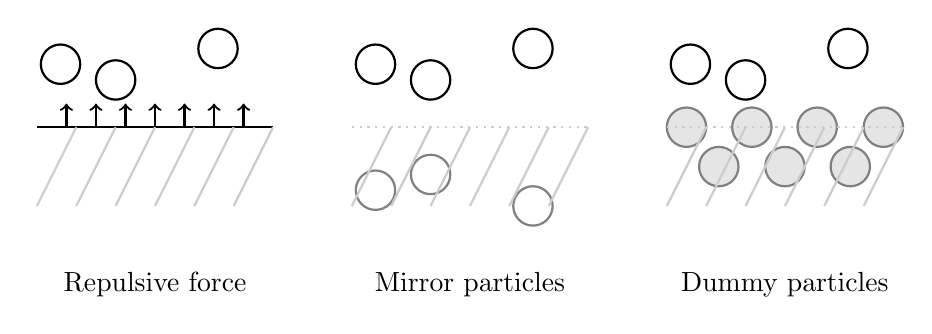
\begin{tikzpicture}[thick]
% Mathematical reflection
\draw (0.3,.8) circle (.25cm) node[pos=.5] (p0) {};
\draw (1,.6) circle (.25cm) node[pos=.5] (p1) {};
\draw (2.3,1) circle (.25cm) node[pos=.5] (p2) {};
\draw (0,0) -- (3,0);
\foreach \i in {1,...,6}{
	\draw[black!20] (.5*\i-.5,-1) -- (.5*\i,0);
}
% Forces
\foreach \i in {1,...,7}{
	\draw[->] (.375*\i,0) -- (.375*\i,.3);
}
\node at (1.5,-2) {Repulsive force};

% Mirror 
\draw (4.3,.8) circle (.25cm) node[pos=.5] (p0) {};
\draw (5,.6) circle (.25cm) node[pos=.5] (p1) {};
\draw (6.3,1) circle (.25cm) node[pos=.5] (p2) {};
\draw[black!50] (4.3,-.8) circle (.25cm) node[pos=.5] (mii1) {};
\draw[black!50] (5,-.6) circle (.25cm) node[pos=.5] (mii2) {};
\draw[black!50] (6.3,-1) circle (.25cm) node[pos=.5] (mii3) {};
\draw[black!20,dotted] (4,0) -- (7,0);
\foreach \i in {1,...,6}{
	\draw[black!20] (.5*\i-.5+4,-1) -- (.5*\i+4,0);
}
\node at (5.5,-2) {Mirror particles};

% Dummies
\draw[black!50,fill=black!10] (8.25,0) circle (.25cm) node[pos=.5] (d0) {};
\draw[black!50,fill=black!10] (9.08,0) circle (.25cm) node[pos=.5] (d1) {};
\draw[black!50,fill=black!10] (9.91,0) circle (.25cm) node[pos=.5] (d2) {};
\draw[black!50,fill=black!10] (10.75,0) circle (.25cm) node[pos=.5] (d3) {};
% second layer
\draw[black!50,fill=black!10] (8.66,-.5) circle (.25cm) node[pos=.5] (d4) {};
\draw[black!50,fill=black!10] (9.50,-.5) circle (.25cm) node[pos=.5] (d5) {};
\draw[black!50,fill=black!10] (10.33,-.5) circle (.25cm) node[pos=.5] (d6) {};
%\draw (1,-.25) circle (.25cm) node[pos=.5] (d4) {};
%normal parts
\draw (8.3,.8) circle (.25cm) node[pos=.5] (p0) {};
\draw (9,.6) circle (.25cm) node[pos=.5] (p1) {};
\draw (10.3,1) circle (.25cm) node[pos=.5] (p2) {};
\draw[dotted,black!20] (8,0) -- (11,0);
\foreach \i in {1,...,6}{
	\draw[black!20] (.5*\i-.5+8,-1) -- (.5*\i+8,0);
}
\node at (9.5,-2) {Dummy particles};
\end{tikzpicture}